\documentclass[fontset=fandol]{ctexart}
\usepackage{amssymb}
\usepackage{amsmath}
\usepackage{geometry} % 控制页面缩放
\usepackage{physics} % 一些方便的命令
\usepackage{booktabs} % 提供\toprule, \bottomrule
\usepackage{float} % 控制浮动体
\usepackage{subcaption} % 子图
\usepackage{fontspec} % 字体选择
\setmonofont{Consolas} % 设置无衬线字体为Consolas
\usepackage[T1]{fontenc}
\usepackage{mathpazo} % 设置Palatino风格的西文字体
\usepackage{graphicx}
\usepackage{enumerate}
\usepackage{enumitem} % 调整列表环境
\usepackage{abstract} % 调整摘要样式
\usepackage{bm}
\usepackage{listings}
\lstset{numbers=left,numberstyle=\small,frame=single,basicstyle=\ttfamily}
\usepackage[hidelinks]{hyperref} % 引入交叉引用
\usepackage{xchoices} % 选择题环境
\usepackage{ulem}
\usepackage{CJKulem} % 自适应下划线
\usepackage{fontawesome} % 对错号,对号\faCheck,错号\faTimes
\usepackage{ntheorem}
\newtheorem*{proof}{解} % 解
\usepackage{circledtext} % 带圈数字
% 对列表环境的设置
\setenumerate[1]{itemsep=0pt,partopsep=0pt,parsep=\parskip,topsep=5pt,listparindent=0em}
\setitemize[1]{itemsep=0pt,partopsep=0pt,parsep=\parskip,topsep=5pt,listparindent=0em}
\numberwithin{equation}{section} % 公式编号依照section
\geometry{a4paper,scale=0.8} % 内容占页面0.8
\renewcommand{\abstractnamefont}{\heiti} % 摘要标题设置为黑体
\setcounter{tocdepth}{1} % 目录深度为1
\newcommand{\fillin}{\uline{\hbox to 10mm{}}}
% xelatex --synctex=1 Boltzmann.tex
\begin{document}

\title{\heiti 格子Boltzmann方法解二维圆柱绕流}

\author{一小块浓缩铀}

\date{\zhtoday}

\maketitle

%\newpage
%\tableofcontents
\newpage
%% 正文部分 %%
\section{LBM方法概述}
LBM全称Lattice Boltzmann Method,即格子玻尔兹曼方法,这是一种介观的(宏观和微观之间的)一种模拟方法,在宏观上是离散方法,微观上是连续方法。此方法边界条件容易处理,得到的物理图像清晰,并行性能好,已经在微尺度流、多孔介质流、湍流和燃烧问题等领域得到广泛应用。
\subsection{Boltzman方程}
任何一个宏观体系中,每个分子的微观运动都遵守力学规律,因此只要计算出大量粒子的个别运动,就可以确定系统的宏观参数;另一方面,我们可以求出每个分子处在某一状态下的概率,通过统计的方法得出系统的宏观参数,这是Boltzmann方程的基本思想。

首先接受三个重要假设:
\begin{enumerate}
    \item 分子相互碰撞时只考虑二体碰撞。
    \item 粒子在碰撞之前速度不相关。
    \item 外力不影响局部碰撞的动力学行为。
\end{enumerate}

设速度分布函数$f$是空间位置矢量$\va*{r}(x,y,z)$、分子速度矢量$\va*{\xi}(\xi_x,\xi_y,\xi_z)$和时间$t$的函数。那么$f(\va*{r},\va*{\xi},t)$表示$t$时刻,在$\va*{r}$到$\va*{r}+\dd{\va*{r}}$间的体积元$\dd{\va*{r}}=\dd{x}\dd{y}\dd{z}$中,速度在$\va*{\xi}$到$\va*{\xi}+\dd{\va*{\xi}}$的分子数。若设$t$时刻,$\va*{r}$处单位体积内的分子数,则
\begin{equation}
    n = \int f(\va*{r},\va*{\xi},t)\dd{\va*{\xi}}
\end{equation}
若分子在时间间隔$\dd{t}$内无碰撞,则只有其位置和速度发生变化,分子的数目保持不变,即
\begin{equation}
    f(\va*{r}+\dd{\va*{r}},\va*{\xi}+\va*{a}\dd{t},t+\dd{t})\dd{\va*{r}}\dd{\va*{\xi}}=f(\va*{r},\va*{\xi},t)\dd{\va*{r}}\dd{\va*{\xi}}
\end{equation}
对上式左端作Taylor展开,两边同时除以$\dd{t}$,并令$\dd{t}\to 0$,则
\begin{equation}
    \pdv{f}{t}+\va*{\xi}\cdot\pdv{f}{\va*{r}}+\va*{a}\cdot\pdv{f}{\va*{\xi}}=0
\end{equation}
由于此时仅考虑了分子的一般运动,而没有考虑碰撞,因此可以写为
\begin{equation}
    \left(\pdv{f}{t}\right)_{\text{运动}}=-\va*{\xi}\cdot\pdv{f}{\va*{r}}-\va*{a}\cdot\pdv{f}{\va*{\xi}}\label{1.4}
\end{equation}
我们认为分子只存在一般运动和碰撞,因此
\begin{equation}
    \pdv{f}{t}=\left(\pdv{f}{t}\right)_{\text{运动}}+\left(\pdv{f}{t}\right)_{\text{碰撞}}\label{1.5}
\end{equation}
联立\ref{1.4}和\ref{1.5},并将碰撞项记为$\varOmega_f$,则\textbf{Boltzmann方程}可表示为
\begin{equation}
    \pdv{f}{t}+\va*{\xi}\cdot\pdv{f}{\va*{r}}+\va*{a}\cdot\pdv{f}{\va*{\xi}}=\varOmega_f
\end{equation}
关于碰撞项$\varOmega_f$的表示和求解比较复杂,下面给出BGK近似下的Boltzmann方程。
\subsection{Boltzmann-BGK方程}
BGK近似下,认为碰撞效应改变$f$使其趋于Maxwell平衡态分布$f^{\rm eq}$,设改变率的大小和$f^{\rm eq}-f$成正比,引入
\begin{equation}
    \varOmega_f=\nu\left[f^{\rm eq}(\va*{r},\va*{\xi})-f(\va*{r},\va*{\xi},t)\right]
\end{equation}
这样得到Boltzmann-BGK方程如下
\begin{equation}
    \pdv{f}{t}+\va*{\xi}\cdot\pdv{f}{\va*{r}}+\va*{a}\cdot\pdv{f}{\va*{\xi}}=\nu\left(f^{\rm eq}-f\right)
\end{equation}
事实上,$\nu$为碰撞频率,$\tau_0=1/\nu$为弛豫时间。
\subsection{格子Boltzmann方法}
要想对Boltzmann-BGK方程使用计算机程序求解,势必要对其进行离散化,格子Boltzmann方程即离散化的Boltzmann-BGK方程,即
\begin{equation}
    \pdv{f_\alpha}{t}+\va*{e}_\alpha\cdot\nabla f_\alpha=-\frac{1}{\tau_0}\left(f_\alpha-f_\alpha^{\rm eq}\right)+\left(\va*{a}\cdot\nabla_{\xi}f\right)_\alpha
\end{equation}
这种离散处理将流体视为大量离散的粒子,每个粒子都会安排在一个规定好的格子Lattice上,并按照格子的规则进行迁移,即碰撞和运动。此时,不仅空间是离散的,时间和速度也是离散的。

LBM的基本模型是\textbf{DdQm}模型($d$维空间,$m$个离散速度),D2Q9是比较常用的一种,示意如下。
\begin{figure}[H]
    \centering
    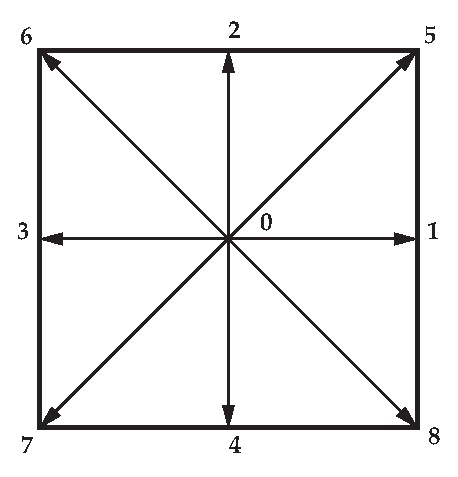
\includegraphics[scale=0.6]{D2Q9.eps}
    \caption{D2Q9模型}
\end{figure}
平衡态分布函数
\begin{equation}
    f_{\alpha}^{\rm eq}=\rho\omega_\alpha\left[1+\frac{\va*{e}_\alpha\cdot \va*{u}}{c_s^2}+\frac{(\va*{e}_\alpha\cdot \va*{u})^2}{2c_s^4}-\frac{u^2}{2c_s^2}\right]
\end{equation}
其中,权重系数
\begin{equation*}
    \omega_\alpha=\begin{cases}
        4/9, &\va*{e}_alpha^2=0\\
        1/9, &\va*{e}_alpha^2=e^2\\
        1/36, &\va*{e}_alpha^2=2e^2
    \end{cases}
\end{equation*}
格子声速$c_s$为常数,离散速度$\va*{e}_\alpha$满足
\begin{equation*}
    \va*{e}_\alpha=e\begin{bmatrix}
        0 & 1 & 0 & -1 & 0 & 1 & -1 & -1 & 1 \\
        0 & 0 & 1 & 0 & -1 & 1 & 1 & -1 & -1 
    \end{bmatrix}
\end{equation*}

因此我们可以通过格子中某一点的宏观速度$\va*{u}$和密度$\rho$,求解出该点的平衡态分布函数$f_{\alpha}^{\rm eq}$,这是重要的宏观参数转化为微观参数的重要步骤。
\end{document}